% !TeX root = ../main.tex

\chapter{建模与验证}

\section{C模型}

% TODO 解释C模型在ASIC设计中的作用                                          
据统计,全世界有67\%以上的ASIC项目都是拖期交付的,其中有些项目会拖期半年以上,从这个数据
可以想象得到,通向一款ASIC芯片的道路会有多么曲折。ASIC芯片的特点与简单指令集的CPU完全相反,
它被设计出来的目的就是为了实现复杂功能。因此,ASIC芯片的设计过程异常繁琐。一般的,芯片公司
会在项目初始时,完成市场需求设计和产品需求设计。在需求被明确之后,系统工程师就会开始进行架构
设计。这个过程包含了提出顶层架构设计和定义需求中所有用例涉及到的子模块。并且,定义各个子模块
之间的连接关系、交互方式和时序要求。
在完成芯片的架构设计之后,需要对芯片进行建模。芯片建模是用一种高级语言对芯片的行为进行描述。
一般会采用C/C++或者SystemC来实现建模。如果涉及到新的算法模块,会要求算法工程师先做出算法的
Matlab或者Python模型,作为模块开发者和芯片模型的参考依据。

\subsection{顶层架构}
在章节2.1中,本文已经简述了总体的架构设计。本章节将详细说明顶层架构的C模型。


\subsection{数据的输入}
需要设计相应的模块处理输入的图像数据,使得神经网络计算模块可以进行计算。
%TODO 描述DVP并口传输input的数据
%DRAFT 设计有下列端口
%       PCLK        像素点同步时钟信号
%       XCLK        外部输入时钟信号
%       VSYNC       帧同步信号
%       HSYNC       行同步信号
%       Data[0:11]  数据信号12bit


%TODO 设计Input Data Adapter
%       buffer      5行buffer


\subsection{数据的运算}  

\subsubsection{脉动阵列的仿真}
% TODO 首先实现脉动和PE
定义处理单元和实现脉动的行为。
\begin{codeblock}[language=C]
#include <iostream>
#include <cstdlib>
#include <ctime>
#include <iomanip>
#define N 256
using namespace std;

typedef struct PE{
    int weight;
    int neuron;
    int psum;
};

class Systolic{
public:
    PE S[N][N];
public:
    void Init(){
        for(int i=0;i<N;i++)
            for(int j=0;j<N;j++){
                S[i][j].psum=0;
                S[i][j].weight=0;
                S[i][j].neuron=0;
            }
    }
    void calc(){
        for(int i=0;i<N;i++)
            for(int j=0;j<N;j++)
                S[i][j].psum+=S[i][j].weight*S[i][j].neuron;
    }
    void shift(int a[N],int b[N]){
        //水平方向传播矩阵A,a[N]是本次要被读入的列(left->right)
        for(int i=0;i<N;i++)
            for(int j=N-1;j>0;j--){
                S[i][j].neuron=S[i][j-1].neuron;
        }
        for(int i=0;i<N;i++)
            S[i][0].neuron=a[i];
        //竖直方向上传播矩阵B,b[N]是本次要被读入的行(up->bottom)
        for(int j=0;j<N;j++)
            for(int i=N-1;i>0;i--){
                S[i][j].weight=S[i-1][j].weight;
        }
        for(int j=0;j<N;j++)
            S[0][j].weight=b[j];
    }
    void Display(){
        cout<<"weight:"<<endl;
        for(int i=0;i<N;i++){
            for(int j=0;j<N;j++)
                cout<<fixed<<setw(4)<<S[i][j].weight<<",";
            cout<<endl;
        }
        cout<<"neuron:"<<endl;
        for(int i=0;i<N;i++){
            for(int j=0;j<N;j++)
                cout<<fixed<<setw(4)<<S[i][j].neuron<<",";
            cout<<endl;
        }
    }
};

\end{codeblock}



% 以下是原来的内容


\begin{figure}[!htp]
  \centering
  
\includegraphics[height=2cm]{sjtu-vi-badge-blue.pdf}
  \hspace{1cm}
  
\includegraphics[height=2cm]{sjtu-vi-badge-blue.pdf}
  \bicaption{中文题图}{English caption}
  \label{fig:SRR}
\end{figure}

如果多个图形相互独立,并不共用一个图形计数器,那么用 \texttt{minipage} 或者
\texttt{parbox} 就可以,如图~\ref{fig:parallel1} 与图~\ref{fig:parallel2}。

\begin{figure}[!htp]
\begin{minipage}{0.48\textwidth}
  \centering
  
\includegraphics[height=1.5cm]{sjtu-vi-name-blue.pdf}
  \caption{并排第一个图}
  \label{fig:parallel1}
\end{minipage}\hfill
\begin{minipage}{0.48\textwidth}
  \centering
  
\includegraphics[height=1.5cm]{sjtu-vi-name-blue.pdf}
  \caption{并排第二个图}
  \label{fig:parallel2}
\end{minipage}
\end{figure}

Lorem ipsum dolor sit amet, consectetur adipisici elit, sed do eiusmod tempor
incididunt ut labore et dolore magna aliqua. Ut enim ad minim veniam, quis
nostrud exercitation ullamco laboris nisi ut aliquip ex ea commodo consequat.
Duis aute irure dolor in reprehenderit in voluptate velit esse cillum dolore eu
fugiat nulla pariatur. Excepteur sint occaecat cupidatat non proident, sunt in
culpa qui officia deserunt mollit anim id est laborum.

如果要为共用一个计数器的多个子图添加子图题,建议使用较新的 \pkg{subcaption}宏
包,不建议使用 \pkg{subfigure} 或 \pkg{subfig} 等宏包。

推荐使用 \pkg{subcaption} 宏包的 \cs{subcaptionbox} 并排子图,子图题置于子图之
下,子图号用 a)、b) 等表示。也可以使用 \pkg{subcaption} 宏包的 \cs{subcaption}
(放在 minipage中,用法同 \cs{caption})。

搭配 \pkg{bicaption} 宏包时,可以启用 \cs{subcaptionbox} 和 \cs{subcaption} 的双
语变种 \cs{bisubcaptionbox} 和 \cs{bisubcaption},如图~\ref{fig:bisubcaptionbox}
所示。

\begin{figure}[!hbtp]
  \centering
  \bisubcaptionbox{$R_3 = 1.5\text{mm}$ 时轴承的压力分布云图}%
                  {Pressure contour of bearing when $R_3 = 1.5\text{mm}$}%
                  [6.4cm]{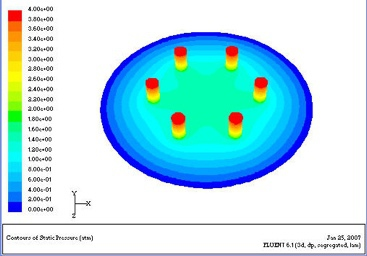
\includegraphics[height=2.5cm]{pressure15.jpg}}
  \hspace{1cm}
  \bisubcaptionbox{$R_3 = 2.5\text{mm}$ 时轴承的压力分布云图}%
                  {Pressure contour of bearing when $R_3 = 2.5\text{mm}$}%
                  [6.4cm]{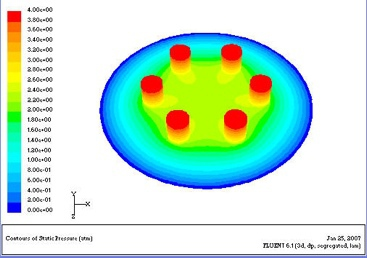
\includegraphics[height=2.5cm]{/pressure25.jpg}}
  \bicaption{包含子图题的范例(使用 subcaptionbox)}
            {Example with subcaptionbox}
  \label{fig:bisubcaptionbox}
\end{figure}

\pkg{subcaption} 宏包也提供了 \pkg{subfigure} 和 \pkg{subtable} 环境,如
图~\ref{fig:subfigure}。

\begin{figure}[!htp]
  \centering
  \begin{subfigure}{0.3\textwidth}
    \centering
    
\includegraphics[height=2cm]{sjtu-vi-badge-blue.pdf}
    \caption{校徽}
  \end{subfigure}
  \hspace{1cm}
  \begin{subfigure}{0.4\textwidth}
    \centering
    
\includegraphics[height=1.5cm]{sjtu-vi-name-blue.pdf}
    \caption{校名。注意这个图略矮些,subfigure 中同一行的子图在顶端对齐。}
  \end{subfigure}
  \caption{包含子图题的范例(使用 subfigure)}
  \label{fig:subfigure}
\end{figure}

Lorem ipsum dolor sit amet, consectetur adipisici elit, sed do eiusmod tempor
incididunt ut labore et dolore magna aliqua. Ut enim ad minim veniam, quis
nostrud exercitation ullamco laboris nisi ut aliquip ex ea commodo consequat.
Duis aute irure dolor in reprehenderit in voluptate velit esse cillum dolore eu
fugiat nulla pariatur. Excepteur sint occaecat cupidatat non proident, sunt in
culpa qui officia deserunt mollit anim id est laborum.

\section{表格}

\subsection{基本表格}

编排表格应简单明了,表达一致,明晰易懂,表文呼应、内容一致。表题置于表上,研究生
学位论文可以用中、英文两种文字居中排写,中文在上,也可以只用中文。

表格的编排建议采用国际通行的三线表\footnote{三线表,以其形式简洁、功能分明、阅读
方便而在科技论文中被推荐使用。三线表通常只有 3 条线,即顶线、底线和栏目线,没有
竖线。}。三线表可以使用 \pkg{booktabs} 提供的 \cs{toprule}、\cs{midrule} 和
\cs{bottomrule}。它们与 \pkg{longtable} 能很好的配合使用。

\begin{table}[!hpt]
  \caption[一个颇为标准的三线表]{一个颇为标准的三线表\footnotemark}
  \label{tab:firstone}
  \centering
  \begin{tabular}{@{}llr@{}} \toprule
    \multicolumn{2}{c}{Item} \\ \cmidrule(r){1-2}
    Animal & Description & Price (\$)\\ \midrule
    Gnat  & per gram  & 13.65 \\
          & each      & 0.01 \\
    Gnu   & stuffed   & 92.50 \\
    Emu   & stuffed   & 33.33 \\
    Armadillo & frozen & 8.99 \\ \bottomrule
  \end{tabular}
\end{table}
\footnotetext{这个例子来自
  \href{https://mirrors.sjtug.sjtu.edu.cn/ctan/macros/latex/contrib/booktabs/booktabs.pdf}%
  {《Publication quality tables in LaTeX》}(\pkg{booktabs} 宏包的文档)。这也是
  一个在表格中使用脚注的例子,请留意与 \pkg{threeparttable} 实现的效果有何不
  同。}

\subsection{复杂表格}

我们经常会在表格下方标注数据来源,或者对表格里面的条目进行解释。可以用
\pkg{threeparttable} 实现带有脚注的表格,如表~\ref{tab:footnote}。

\begin{table}[!htpb]
  \bicaption{一个带有脚注的表格的例子}{A Table with footnotes}
  \label{tab:footnote}
  \centering
  \begin{threeparttable}[b]
     \begin{tabular}{ccd{4}cccc}
      \toprule
      \multirow{2}*{total} & \multicolumn{2}{c}{20\tnote{a}} & \multicolumn{2}{c}{40} & \multicolumn{2}{c}{60} \\
      \cmidrule(lr){2-3}\cmidrule(lr){4-5}\cmidrule(lr){6-7}
      & www & \multicolumn{1}{c}{k} & www & k & www & k \\ % 使用说明符 d 的列会自动进入数学模式,使用 \multicolumn 对文字表头做特殊处理
      \midrule
      & $\underset{(2.12)}{4.22}$ & 120.0140\tnote{b} & 333.15 & 0.0411 & 444.99 & 0.1387 \\
      & 168.6123 & 10.86 & 255.37 & 0.0353 & 376.14 & 0.1058 \\
      & 6.761    & 0.007 & 235.37 & 0.0267 & 348.66 & 0.1010 \\
      \bottomrule
    \end{tabular}
    \begin{tablenotes}
    \item [a] the first note.% or \item [a]
    \item [b] the second note.% or \item [b]
    \end{tablenotes}
  \end{threeparttable}
\end{table}

Lorem ipsum dolor sit amet, consectetur adipisici elit, sed do eiusmod tempor
incididunt ut labore et dolore magna aliqua. Ut enim ad minim veniam, quis
nostrud exercitation ullamco laboris nisi ut aliquip ex ea commodo consequat.
Duis aute irure dolor in reprehenderit in voluptate velit esse cillum dolore eu
fugiat nulla pariatur. Excepteur sint occaecat cupidatat non proident, sunt in
culpa qui officia deserunt mollit anim id est laborum.

如某个表需要转页接排,可以用 \pkg{longtable} 实现。接排时表题省略,表头应重复书
写,并在右上方写“续表 xx”,如表~\ref{tab:performance}。

\begin{longtable}[c]{c*{6}{r}}
  \bicaption{实验数据}{Experimental data}
  \label{tab:performance} \\
  \toprule
  测试程序 & \multicolumn{1}{c}{正常运行} & \multicolumn{1}{c}{同步}
    & \multicolumn{1}{c}{检查点} & \multicolumn{1}{c}{卷回恢复}
    & \multicolumn{1}{c}{进程迁移} & \multicolumn{1}{c}{检查点} \\
   & \multicolumn{1}{c}{时间 (s)} & \multicolumn{1}{c}{时间 (s)}
    & \multicolumn{1}{c}{时间 (s)} & \multicolumn{1}{c}{时间 (s)}
    & \multicolumn{1}{c}{时间 (s)} &  文件(KB)\\
  \midrule
  \endfirsthead
  \multicolumn{7}{r}{续表~\thetable} \\
  \toprule
  测试程序 & \multicolumn{1}{c}{正常运行} & \multicolumn{1}{c}{同步}
    & \multicolumn{1}{c}{检查点} & \multicolumn{1}{c}{卷回恢复}
    & \multicolumn{1}{c}{进程迁移} & \multicolumn{1}{c}{检查点} \\
   & \multicolumn{1}{c}{时间 (s)} & \multicolumn{1}{c}{时间 (s)}
    & \multicolumn{1}{c}{时间 (s)} & \multicolumn{1}{c}{时间 (s)}
    & \multicolumn{1}{c}{时间 (s)}&  文件(KB)\\
  \midrule
  \endhead
  \hline
  \multicolumn{7}{r}{续下页}
  \endfoot
  \endlastfoot
  CG.A.2 & 23.05 & 0.002 & 0.116 & 0.035 & 0.589 & 32491 \\
  CG.A.4 & 15.06 & 0.003 & 0.067 & 0.021 & 0.351 & 18211 \\
  CG.A.8 & 13.38 & 0.004 & 0.072 & 0.023 & 0.210 & 9890 \\
  CG.B.2 & 867.45 & 0.002 & 0.864 & 0.232 & 3.256 & 228562 \\
  CG.B.4 & 501.61 & 0.003 & 0.438 & 0.136 & 2.075 & 123862 \\
  CG.B.8 & 384.65 & 0.004 & 0.457 & 0.108 & 1.235 & 63777 \\
  MG.A.2 & 112.27 & 0.002 & 0.846 & 0.237 & 3.930 & 236473 \\
  MG.A.4 & 59.84 & 0.003 & 0.442 & 0.128 & 2.070 & 123875 \\
  MG.A.8 & 31.38 & 0.003 & 0.476 & 0.114 & 1.041 & 60627 \\
  MG.B.2 & 526.28 & 0.002 & 0.821 & 0.238 & 4.176 & 236635 \\
  MG.B.4 & 280.11 & 0.003 & 0.432 & 0.130 & 1.706 & 123793 \\
  MG.B.8 & 148.29 & 0.003 & 0.442 & 0.116 & 0.893 & 60600 \\
  LU.A.2 & 2116.54 & 0.002 & 0.110 & 0.030 & 0.532 & 28754 \\
  LU.A.4 & 1102.50 & 0.002 & 0.069 & 0.017 & 0.255 & 14915 \\
  LU.A.8 & 574.47 & 0.003 & 0.067 & 0.016 & 0.192 & 8655 \\
  LU.B.2 & 9712.87 & 0.002 & 0.357 & 0.104 & 1.734 & 101975 \\
  LU.B.4 & 4757.80 & 0.003 & 0.190 & 0.056 & 0.808 & 53522 \\
  LU.B.8 & 2444.05 & 0.004 & 0.222 & 0.057 & 0.548 & 30134 \\
  EP.A.2 & 123.81 & 0.002 & 0.010 & 0.003 & 0.074 & 1834 \\
  EP.A.4 & 61.92 & 0.003 & 0.011 & 0.004 & 0.073 & 1743 \\
  EP.A.8 & 31.06 & 0.004 & 0.017 & 0.005 & 0.073 & 1661 \\
  EP.B.2 & 495.49 & 0.001 & 0.009 & 0.003 & 0.196 & 2011 \\
  EP.B.4 & 247.69 & 0.002 & 0.012 & 0.004 & 0.122 & 1663 \\
  EP.B.8 & 126.74 & 0.003 & 0.017 & 0.005 & 0.083 & 1656 \\
  SP.A.2 & 123.81 & 0.002 & 0.010 & 0.003 & 0.074 & 1854 \\
  SP.A.4 & 51.92 & 0.003 & 0.011 & 0.004 & 0.073 & 1543 \\
  SP.A.8 & 31.06 & 0.004 & 0.017 & 0.005 & 0.073 & 1671 \\
  SP.B.2 & 495.49 & 0.001 & 0.009 & 0.003 & 0.196 & 2411 \\
  SP.B.4 & 247.69 & 0.002 & 0.014 & 0.006 & 0.152 & 2653 \\
  SP.B.8 & 126.74 & 0.003 & 0.017 & 0.005 & 0.082 & 1755 \\
  \bottomrule
\end{longtable}

\section{算法环境}

算法环境可以使用 \pkg{algorithms} 宏包或者较新的 \pkg{algorithm2e} 实现。
算法~\ref{algo:algorithm} 是一个使用 \pkg{algorithm2e} 的例子。关于排版算法环境
的具体方法,请阅读相关宏包的官方文档。

\begin{algorithm}[htb]
  \caption{算法示例}
  \label{algo:algorithm}
  \small
  \SetAlgoLined
  \KwData{this text}
  \KwResult{how to write algorithm with \LaTeXe }

  initialization\;
  \While{not at end of this document}{
    read current\;
    \eIf{understand}{
      go to next section\;
      current section becomes this one\;
    }{
      go back to the beginning of current section\;
    }
  }
\end{algorithm}

\section{代码环境}

我们可以在论文中插入算法,但是不建议插入大段的代码。如果确实需要插入代码,建议使
用 \pkg{listings} 宏包。

\begin{codeblock}[language=C]
#include <stdio.h>
#include <unistd.h>
#include <sys/types.h>
#include <sys/wait.h>

int main() {
  pid_t pid;

  switch ((pid = fork())) {
  case -1:
    printf("fork failed\n");
    break;
  case 0:
    /* child calls exec */
    execl("/bin/ls", "ls", "-l", (char*)0);
    printf("execl failed\n");
    break;
  default:
    /* parent uses wait to suspend execution until child finishes */
    wait((int*)0);
    printf("is completed\n");
    break;
  }

  return 0;
}
\end{codeblock}
